%\chapter{Eliminating The Impossible, Whatever Remains Must Be True}\label{chap:aaai23}
\chapter{Extracting and Applying Background Knowledge in the Context of Formal Explanations}
\label{chap:aaai23}

This chapter is based on:
\begin{itemize}
	\item Jinqiang Yu, Alexey Ignatiev, Peter J. Stuckey, Nina Narodytska, and Joao Marques-Silva.
Eliminating the impossible, whatever remains must be true: On extracting and applying background
knowledge in the context of formal explanations. \emph{In Proceedings of the AAAI Conference on Artificial
Intelligence,} vol. 37, pp. 4123-4131, 2023.
\end{itemize}

While the formal explainability method provides provably correct and minimal explanations,
a few limitations have been identified.
%
For instance, to ensure provable correctness of explanations, formal methods must consider the entire feature space, 
assuming that features are uniformly distributed and independent~\cite{kutyniok-jair21}.
%
This requires a formal reasoner to examine all potential combinations of feature values, 
even those that are unlikely to occur in practical contexts.
%
While this ensures the correctness of abductive explanations~(AXp's), it may result in unnecessarily
long explanations.
%
Additionally, it raises concerns about the validity of contrastive explanations~(CXp's), 
as the counterexamples they depend on may be not meaningful.
%
Inspired by the limitation, this chapter is aimed at generating both AXp's and CXp's
using background knowledge and presents the following contributions.
%
First, this chapter introduces an efficient method to mine background 
knowledge represented by precise if-then rules for a given training
dataset.
%
This method builds on a recent technique to learn decision 
sets~\cite{ilsms-aaai21}.
%
Second, we presents a novel method to produce AXp's and CXp's subject to extracted background knowledge. 
%
Also, this chapter theoretically demonstrates that incorporating background knowledge 
enhances the quality of both AXp's and CXp's, and therefore helps establish trust in the underlying AI systems.
%
Finally, inspired by~\cite{ignatiev-ijcai20}, we argue that background knowledge 
facilitates a more precise assessment of the correctness of model-agnostic 
explainers by preventing the consideration of impossible combinations of feature values.


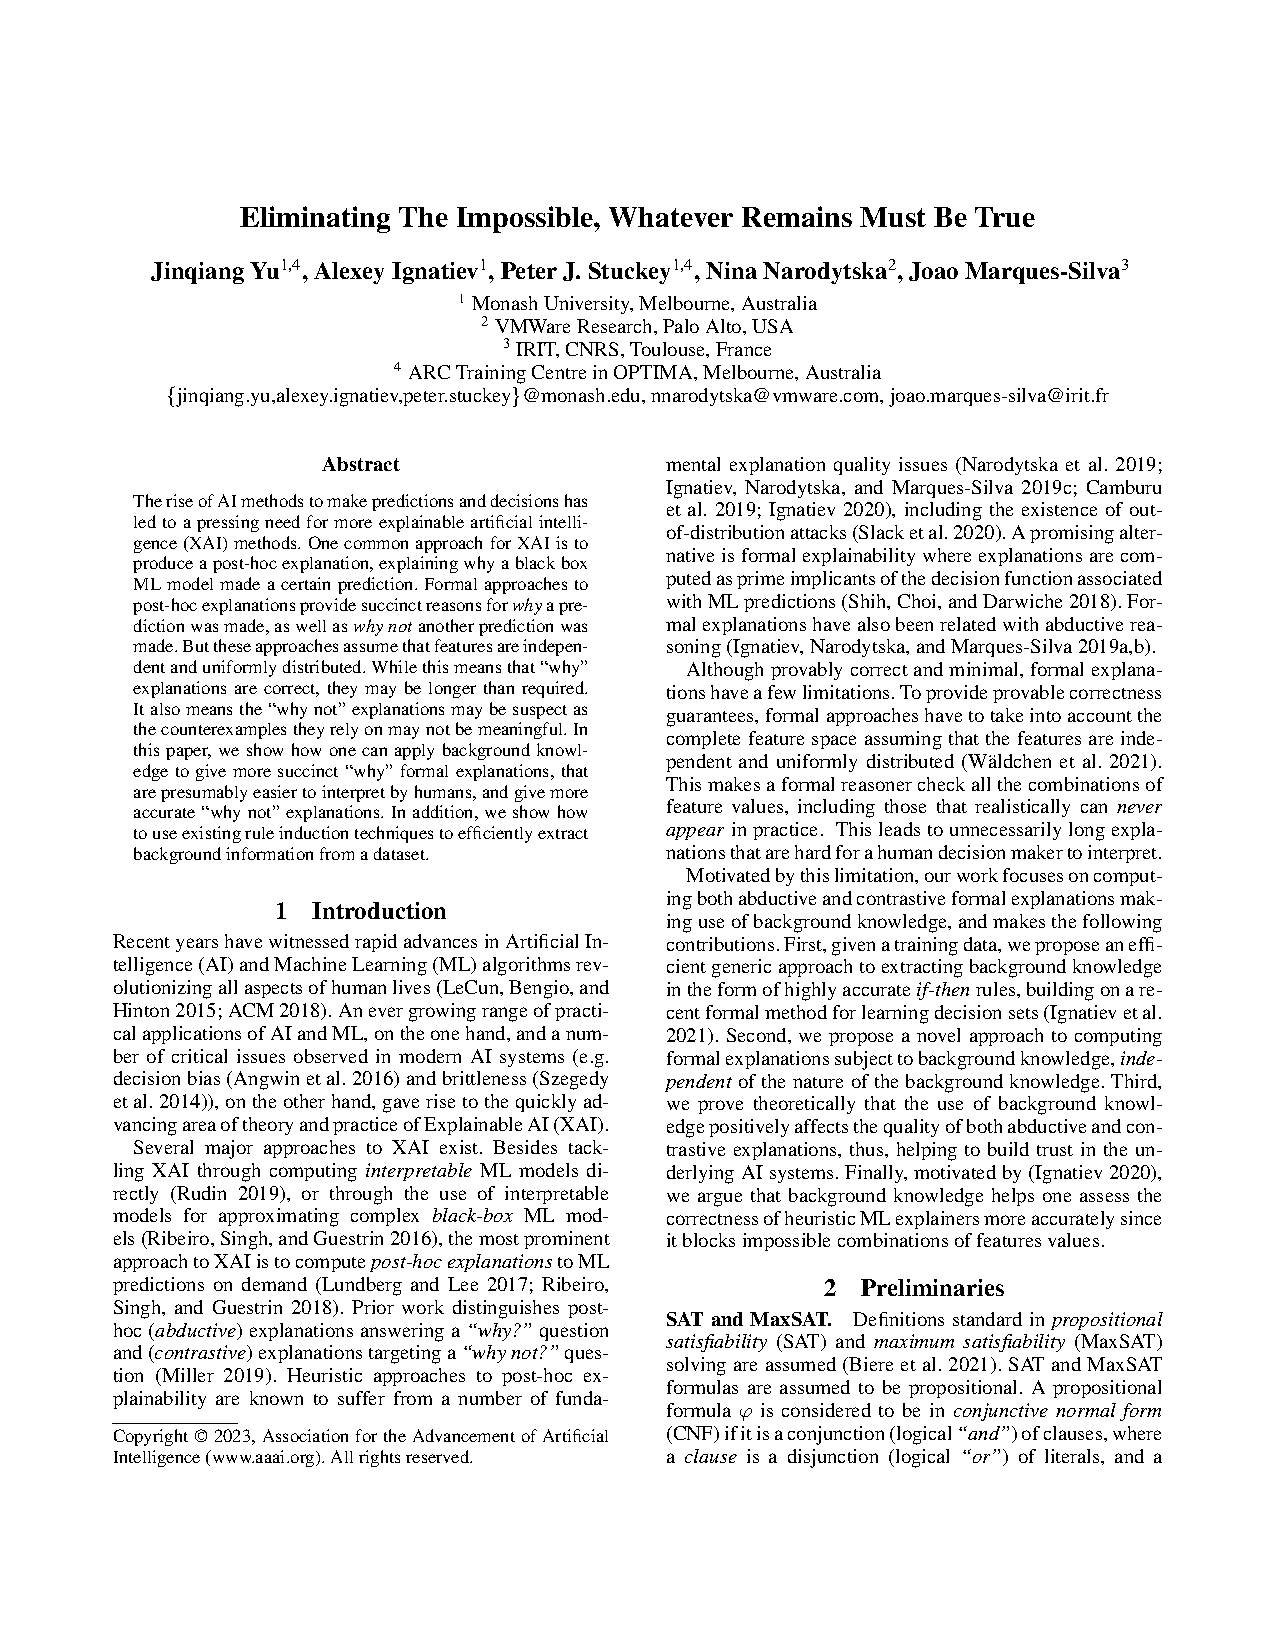
\includepdf[pages=-, offset=75 -75]{papers/aaai23.pdf}
